\section{Theoretical work}\label{sec:theory}

In this section we will present our theoretical work towards exploring the group announcement operator in GAL. In doing this, we will be building on the definitions that were established and introduced in the previous section.

\subsection{Enumeration of announcements in single agent cases}

Going back to the definition of the semantics behind $\M,s \models \dia{G}\varphi$ in Definition \ref{def:dual}, an informal way of explaining it would be that there exists at least one set of formulas the coalition can announce such that $\varphi$ is true after their announcements. 

Using our definitions of labeling formulas and formula extensions in Definition \ref{def:ext} and \ref{def:label} to look at what kinds of formulas any given agent can announce, we note that the goal is to convey information to the other agents in the system. Therefore we do not need to look at the formulas themselves, but only at what consequence announcing them would have and whether or not the agent is able to announce them. For this reason we will be using the concept of formula extensions from Definition \ref{def:ext} rather then concrete formulas as announcing any given formula will eliminate all states not in that formula's extension from the updated model as defined by the semantics of model updates.

\begin{figure}[h]
	\label{fig:GAexample}
	\caption{A basic model with no internally bisimilar states}
	\centering
	\scalebox{1.8}{
		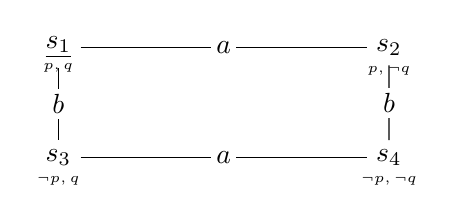
\begin{tikzpicture}[scale = 1.4, every label/.append style = {font=\tiny}]	
				\node[label={[label distance=-0.7cm]:$p,q$}] (s1) at (0,1) {$\underline{s_1}$};
				\node[label={[label distance=-0.7cm]:$p, \neg q$}] (s2) at (3,1) {$s_2$};
				\node[label={[label distance=-0.7cm]:$\neg p, q$}] (s3) at (0,0) {$s_3$};
				\node[label={[label distance=-0.7cm]:$\neg p, \neg q$}] (s4) at (3,0) {$s_4$};
	
				\path[every node/.append style={font=\fontsize{10}{0}, fill=white, inner sep=2pt}] 
					(s1) edge node {$a$} (s2) ++
					(s3) edge node {$a$} (s4) ++
					(s1) edge node {$b$} (s3) ++
					(s2) edge node {$b$} (s4);								
		\end{tikzpicture}
	} %End scaling
\end{figure}

If we attempt to determine which sets of formulas some agent $i$ can announce in the model in Figure \ref{fig:GAexample} we can see that the set of announceable formula extensions will always be a subset of the power set of states in the model. Or more precisely, the set of announceable formula extensions for some agent $i$ in a given pointed model $\M,s$ is a subset of the power set of states in $\M$, where each set is announceable by $i$ if and only if that set follows the following rules in Definition \ref{def:extRules}.

%subset of the power set of extensions of the set of labeling formulas for the model

\begin{definition}[Rules for eliminating formulas by their extension]\hfill
\label{def:extRules}
	For any formula $\varphi$ and bisimulation contracted pointed model $\M,s$, the formula's extension in $\M$, $\ext{\varphi}_{\M}$ must satisfy the following rules in order for the formula to be announceable by some agent $i$ in coalition $G$:
	\begin{itemize}
		\item $\ext{\varphi}_\M$ must contain the actual state in our pointed model
		\item $\forall s\in\ext{\varphi}_{\M}, \forall t\rels_i s \Rightarrow t\in\ext{\varphi}_{\M}$
	\end{itemize}
\end{definition}

The reasoning behind these two rules is that looking back at the semantics of the group announcement operators in Definition \ref{def:GALsem}, we can see that we are essentially searching for a combination of formulas, which when announced will make $\varphi$ false. Because of this, having an agent  announce that they knows something which is false, or something they do not actually know, will simply make the public announcement trivially true. This means there is no point in checking any announcement containing such a formula, therefore the formula:

\begin{itemize}
	\item[(1)] has to be satisfied in the `current' state of our pointed model
	\item[(2)] has to be satisfied in every state the agent is incapable of distinguishing from that `current' state
\end{itemize}

\begin{proposition}
For every extension $\ext{\varphi}_{\M}$ that satisfies the rules in Definition \ref{def:extRules} for some agent, any formula with the same extension can be announced by that agent
\end{proposition}

The reasoning behind this proposition is based on our definition of formula extensions. The extension of a formula is simply the set of states in which this formula is satisfied. Therefore if $\varphi$ and $\psi$ share the same extension in some model $\M$, then $\M\models\varphi \leftrightarrow \psi$. From this we can further infer that $\M\models K_a\varphi \leftrightarrow K_a\psi$ for every $\psi$ with the same extension as $\varphi$


\begin{definition}[The set of announceable extensions]\hfill\\
	\label{def:annexts}
	The set of announceable formula extensions $\anns{}$ for some agent $i$, given a pointed model $\M,s$ is defined 			as the following: \\
	$\anns{i,(\M,s)} \subseteq \wp(\{\ext{\varphi}_{\M} ~|~ \varphi\in\labels{\M}\})$ where $\ext{\varphi}_\M \in 		     
	\anns{i,(\M,s)}$ iff it follows the rules in Definition \ref{def:extRules}.
	Note that since every formula in $\labels{\M}$ is only satisfied in a single state in $\states$, $\wp(\{||\varphi||_\M ~|~ \varphi \in \labels{\M}\})$ can be simplified to $\wp(\states)$.
\end{definition}

For a more practical explanation we will apply these rules to the model in Figure \ref{fig:GAexample} for agent $a$. Using $s_1$ as the actual state of our pointed model, we start by generating the power set of states in our model and get the following:

\begin{align*}
	\wp(\states) = \{\emptyset,\{1\}\{2\},\{3\},\{4\},\{1,2\},...,\{1,2,3\},...\{1,2,3,4\}\}
\end{align*}
After applying rule (1) from Definition \ref{def:extRules}	to filter out all formula extensions not containing the actual state of our pointed model we get:
\begin{align*}
	\{\{1\},\{1,2\},\{1,3\},\{1,4\},\{1,2,3\},\{1,2,4\},\{1,3,4\},\{1,2,3,4\}\}
\end{align*}
Applying rule (2) to remove all extensions relating to formulas that $a$ does not know leaves us with:
\begin{align*}
	\{\{1,2\},\{1,2,3,4\}\}
\end{align*}

In other words, given the model in Figure \ref{fig:GAexample} agent $a$ is able to announce any given formula $\varphi$ iff $\ext{\varphi}_{\M,1} \in \{\{1,2\},\{1,2,3,4\}\}$. Therefore, $\anns{a,(\M,1)} = \{\{1,2\},\{1,2,3,4\}\}$.

An interesting thing to note here is that we can combine our labeling formulas with disjunctions to create a formula which is satisfied in any subset of the original set of states we want. So for example, in order to create a formula with the extension of $\{s_1,s_2\}$ all we have to do is put disjunctions between the labeling formulas for $s_1$ and $s_2$ such that $\varphi_{\{s_1,s_2\}} = \varphi_{s_1} \vee \varphi_{s_2}$.

If we then want to apply this to checking whether $\M,s_1 \models \dia{a}K_bp$ where $\M$ is still the model in Figure \ref{fig:GAexample} then we can see that since $\{s_1,s_2\}\in\anns{a,(\M,s_1)}$ there exists a formula extension that $a$ can announce which would eliminate $s_3$ from the model. This would cause $K_bp$ to be satisfied in the updated model and therefore satisfy $\dia{a}K_bp$.

\subsection{Generalizing the single agent case}

Expanding what we have presented so far to encompass coalitions comprised of multiple agents is actually very easy. 
When we are assessing the ability of an agent to announce something which may change the valuation of a formula, we are simply checking whether or not that agent is capable of eliminating certain states in the updated model. In other words, if we wish to assess the ability of a whole coalition, all we need to do is look at which sets of states each agent in the coalition is able to eliminate in unison.

An interesting observation to make is that an agent $i$ is always capable of eliminating any state they can distinguish from the actual state of some pointed model. This means that in order to find out which states a coalition can eliminate, we can simply take the power set of states and limit it to the combinations of states which fit the rules of Definition \ref{def:extRules}, where we slightly tweak rule 2 to the following:

\begin{definition}[The set of extensions announceable by coalitions]
	\label{def:extscoal}
	The set of announceable extensions $\anns{G,(\M,s)}$ for some coalition $G$, given a bisimulation contracted pointed model $\M,s$ is defined as the following: \\
	$\anns{G,(\M,s)} = \{\states' \subseteq \states ~|~ \forall s'\in \states', \neg\exists t\forall i\in G t\rels_i s', t\not\in \states' \textrm{ and } s\in\states'\}$
\end{definition}


\subsection{Comparison to definitions in original paper on GAL}

\todo{reword intro}

In this section we will compare our definitions and work so far with the definitions presented by Ågotnes et al. in their paper on GAL. In their paper they describe how to check formulas of the kind $\dia{G}\varphi$ in the following manner:

\begin{definition}[Definition of $\dia{G}\varphi$ by Ågotnes et al.]
	\label{def:GALsemAagotnes}
	$\M,s\models \dia{G}$ iff there is a definable restriction $\M'' = (\states'',\rels'',V')$ of $\M$  such that $\states'' = \cap_{i\in G}C_i$ where  $C_i$  are unions of classes of equivalence for $\rels_i$ and $s\in\states''$ and $\M',s\models\varphi$
\end{definition}

Decomposing their definition we end up with $\states''$ being the intersection of the unions of some subset of each agent's equivalence relation. More specifically, for each agent $i$, we choose which equivalence classes 
should be part of that agent's union of equivalence classes $C_i$ and then check if there exists some combination of values for each $C_i$ such that restricting the set of states to the intersection of these $C_i$s gives us a model which both contains the original state $s$ and satisfies $\varphi$.

Comparing this definition to our definition of the announceable set of extensions for a coalition, we argue that our definition of $\anns{G,(\M,s)}$ defines exactly these intersections of possible combinations of $C_i$s from the definition of Ågotnes et al. If we further decompose their definition, we end up with the two following restrictions:
\begin{align}
	&S'' = \bigcap_{i\in G}C_i \textrm{ where } C_i \subseteq S, \forall s\in C_i, \eqc{s}_i\subseteq C_i \\
	&s \in S''
\end{align}

From this, we argue that our definition of $\anns{G,(\M,s)}$ incorporates the same two restrictions, in turn quantifying the set of all possible restricted sets $\states''$. Decomposing our definition the same way we did Definition \ref{def:GALsemAagotnes}, we end up with $\anns{G,(\M,s)}$ defined as the set of all subsets of $\states$, $S'$ which satisfy the following two restrictions:
\begin{align}
	&\forall s'\in S' \neg\exists t\forall i \in G, t\rels_i s', t\not\in S' \\
	&s\in S'
\end{align}

Expanding on our restriction in $(3)$, we could write it out as `if there exists a state $t$ indistinguishable by all agents from $s$, then either $t\in S'$ or $s\not\in S'$'. A simpler way of phrasing this would be to say that for every state in $S'$, the intersection of it's equivalence classes for all agents in the coalition has to be a subset of $S'$. Changing (3) to fit this simpler phrasing gives us
\begin{align}
	\forall s'\in S' \cap_{i\in G}\eqc{s'}_i\subseteq S'
\end{align}

which should further clarify that combining restriction $(4)$ and $(5)$ provides the same set of possible values as $(1)$ and $(2)$. Based on this, we revise the semantics for the group announcement operators into the following:

\begin{definition}[Group announcement operators, revised]
	\label{def:GALsemV2}
	\begin{align*}
		\M,s & \models [G]\varphi \textrm{ iff }  \forall Ext\in\anns{G,(\M,s)} \textrm{ then } \M,s\models [\varphi_{Ext}]\varphi\\
		\M,s & \models \dia{G}\varphi \textrm{ iff } \exists Ext\in\anns{G,(\M,s)} \textrm{ such that } \M,s\models \dia{\varphi_{Ext}}\varphi
	\end{align*}
	Where $\varphi_{Ext}$ is a formula of the form $\bigvee_{s\in Ext}\varphi_{s}$
\end{definition}

Our reasons for this revised definition is that the original definition in \ref{def:GALsem} defines satisfaction of $[G]\varphi$ using a quantifier over an infinite set of formulas making it unfit for our goals of implementing a model checking tool. We will therefore be implementing the revised definition in \ref{def:GALsemV2} instead as the set of announceable extensions is far easier to enumerate than the set of announceable formulas. This is still equivalent to the original definition as we are simply grouping the infinite set of announceable formulas into a finite set of announceable extensions.

\todo{Walk through example of using updated definition to generate set of announceable extensions for coalition based on previous example and model}